\documentclass[journal,sort]{IEEEtran}

\usepackage{lineno,hyperref}
\usepackage{bm}
\usepackage{cancel}
\usepackage{booktabs}
\usepackage{multirow}
\usepackage{array,chngpage}
\usepackage{subfigure}
\usepackage{amssymb}
\usepackage{graphicx}
\usepackage{amsmath}
\usepackage{bm}
\usepackage{diagbox}
\usepackage{cite}
\usepackage{threeparttable}
\usepackage{url}
\usepackage{setspace}
\usepackage{caption}
\DeclareMathOperator*{\argmax}{argmax}
\usepackage[linewidth=1pt]{mdframed}
\usepackage{lipsum}
\usepackage{booktabs}
\usepackage{color}
\usepackage{longtable}
\usepackage{algorithm}


\bibliographystyle{IEEEtran}

\begin{document}

\title{Adaptive and Generative Intra-frame Steganography in HEVC Video Using the Intra Block Partitioning Structure}
\author{XXXX}
	

\maketitle

\begin{abstract}
Intra-frame steganography in HEVC video is a challenge task in the field of video steganography.In this paper, steganographic characteristic of HEVC intra block partitioning structure is first analyzed. It is proved that visual quality of stego video tends to become nearly unchanged after modifying intra block partitioning structure, but the coding efficiency and security of stego video will be affected to some extent.
Based on this property, a novel steganography method based on intra block partitioning structure is proposed to embed the secret payload. In the proposed method, the secret message is not embedded into videos by modifying the cover, but is utilized to generate the cover by a generator. The cover generator can generate four different kinds of intra block partitioning structure with different depth to make full use of HEVC intra-coding structure for high-efficient video steganography.To minimize the potiential statistical detectability, an adaptive matching scheme is designed to use the appropriate generated cover for different video content.
The proposed method is examined on HD video database with different resolution and video contents,and results are further compared with previous Intra-frame steganography method to confirm the effectiveness and advantages of this method. Results also prove that compared to the traditional intra-frame cover, the intra prediction modes, the intra block partitioning structure is a more efficient and secured intra-frame hidden cover for HEVC video.


	
	
\end{abstract}	
\begin{IEEEkeywords}
		video steganography, HEVC, block partitioning structure, generative steganography
\end{IEEEkeywords}
	
\section{Introduction\label{intro}}

As an important method to ensure communication security in the network environment, Steganography has always been a key, cutting-edge research area. Steganography utilizes the characteristics of massive data exchange in the Internet, constructs a hidden channel that humans cannot detect, and transmits a large amount of secret information. This technology is both a new opportunity and a new challenge for the security communication.


One of the most challenge research task in steganography is video steganography. As a carrier of large capacity, high concealment, redundant space diversity and robustness, video has more theoretical research significance and value than image and audio steganography. Taking HEVC coded video as an example, the coding standard designed for high-definition video, the amount of data of high-definition video itself is huge, and its coding technology also brings a new coding domain steganography space, in technical complexity, algorithm security and hidden The diversity of write space is more suitable for security information steganography.

Many works have been done in both H.264/AVC and HEVC [3, 4]. Hu et al. [5] proposed a steganographic algorithm based on intra prediction mode in H.264/AVC. Yang et al. [6] have improved Hu’s method by matrix coding. Bou-chama [7] divided the intra prediction modes in H.264/AVC into four groups ac-cording to their prediction direction, the result shows a better video quality while ensuring high capacity. Zhang et al. [8] analyzed the texture of the video, and pro-posed a high security adaptive embedding algorithm using STC. Wang et al. [9] proposed intra prediction mode based method for HEVC, a mapping between an-gle difference and secret message was established to embed data. Dong et al. [10] further proposed the prediction mode steganography technology under the HEVC standard, and made a breakthrough in the capacity limitation of the previous HEVC intra prediction mode based algorithm, while also improving the security.

The contribution of  this paper including:1) a novel cover generator is proposed to 


The rest of this paper is organized as follows: In Section
2, the Steganographic characteristic of HEVC intra quadtree partition structure is described. In Section 3, the
The proposed Steganographic method for HEVC incluing the cover geneator and the mathing scheme is presented.
Section 4 gives the framework of the proposed method. Section 5 describes the experiments and results analysis for
HEVC videos. Section 5 draws the conclusion.
\section{Steganographic characteristic of Intra Block Partitioning Structure in HEVC}
In this section, the HEVC intra block partitioning structure will be first described, with which distortion analysis of visual quality, coding efficiency and security in HEVC intra steganographic algorithm can be thoroughly introduced next.
\subsection{Intra Block Partitioning Structure in HEVC }
As in all prior ITU-T and ISO/IEC JTC 1 video coding
standards since H.261, the HEVC design follows the
classic block-based hybrid video coding approach. The basic source-coding algorithm is a hybrid
of interpicture prediction to exploit temporal statistical dependences,
intrapicture prediction to exploit spatial statistical
dependences, and transform coding of the prediction residual
signals to further exploit spatial statistical dependences[].Compared with the previous coding standards, HEVC proposes and adopts some new coding technologies based on  the classic block-based hybrid coding approach. With the introduction of these new technologies, the coding efficiency of HEVC has been greatly improved. The intra quadtree block partitioning structure is one of these key technologies.


\begin{figure}[htbp!]
	\centering
	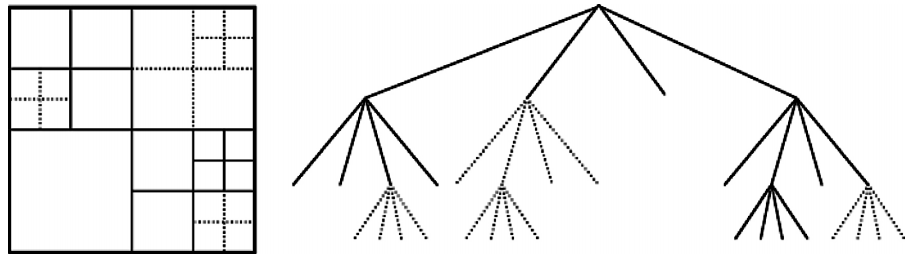
\includegraphics[width=0.5\textwidth]{1.png}
	\caption{HEVC intra partitioning structure}
	\label{HEVC-part}
\end{figure}
The HEVC standard has adopted a highly flexible and efficient intra block partitioning structure. Frames are splited into an integer multiple of CTU, which is an analogous term to the macroblock in H.264/AVC. A CTU consists of one luminance CTB and two chrominance CTB.The terms coding
tree block (CTB) is defined to specify the 2-D sample array of one color component associated with the CTU. In the CTU, a quadtree is established. Let CTU size be 2N$\times$2N where N is one of the values of 32, 16, or 8. The CTU can be further recursively split into four smaller units of equal sizes of N$\times$N, which are nodes of the quadtree. If the
units are leaf nodes of the quadtree, the units become coding units (CUs).

\begin{figure}[htbp!]
	\centering
	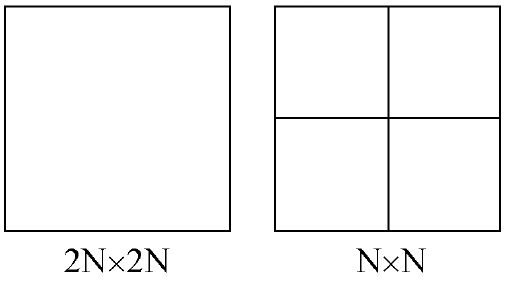
\includegraphics[width=0.2\textwidth]{2.png}
	\caption{HEVC intra partitioning structure}
	\label{HEVC-part}
\end{figure}

HEVC utilizes CU as a unit to specify which prediction
scheme is used for intra and inter predictions. One or more PUs are specified for each CU, which is
a leaf node of coding tree. Coupled with the CU, the PU
works as a basic representative block for sharing the prediction
information.A CU can be split into one ,two or four PUs according to
the PU splitting type. HEVC defines two splitting shapes for
the intra coded CU.Similar to prior standards, each CU
in HEVC can be classified into three categories: skipped CU,
inter coded CU, and intra coded CU.For the intra coded CU, two possible
PU splitting types of PART2N$\times$2N and PARTN$\times$N
are supported.

A CU may be divided into one or more TUs. TU is the basic unit of transform and quantization, and For each
TU, one integer transform having the same size to the TU is applied to obtain residual coefficients. Starting from the CU size, the TU is equally divided in an iterative manner, and whether it is divided into four sub-blocks is calibrated according to the syntax element split transform flag. The size of one TU may be one of 32$\times$32, 16$\times$16, 8$\times$8, and 4$\times$4 depending on the depth of the iteration partition.


In general, in the HEVC standard, the intra-recursive blocking process is as follows: starting from the root node of the quadtree, for a 2NX2N CU, the intra prediction is performed with the current depth as a whole. Calculate its intra prediction direction and the corresponding rate distortion cost. If the CU can continue to divide the leaf nodes, the same prediction process is performed on the four leaf node CUs that are divided, and the intra prediction direction and the corresponding rate distortion cost are calculated. Finally, the cost of different blocking modes is preserved from the root node of the quadtree to the leaf node. Then, starting from the root node, pruning layer by layer, comparing the rate distortion cost of four small CUs plus the rate distortion cost of the CU after a partitioning cost and a parent node, and finally forming a complete block structure of the CTU.


According to the above blocking process,the coding tree approach in HEVC can bring additional coding efficiency benefits by incorporating PU and TU quadtree concepts for video compression. it is obvious that if we modify the block structure in a CTU, it will affect its corresponding rate distortion cost, prediction direction and other coding parameters, thus the visual quality, coding efficiency, and parameter statistics of the video. Characteristics have an impact. Therefore, we will separately analyze the impact of the above three parts after modifying the block structure.


\subsection{Distortion Analysis on visual quality}
We first provide an example to illustrate the visual quality changes after modifying the blocking mode. In the figure, a represents unmodified HEVC video, b represents HEVC video with cu block mode all 32x32, c represents HEVC video with cu block mode all 16x16, and d represents cu block mode all 8x8 HEVC video. We compare the picture quality difference between bcd and a by SSIM value. The SSIM formula is as follows:
\begin{equation}
\delta SSIM=SSIM(A)-SSIM(B) 
\end{equation}
The above phenomenon is caused by the intra prediction and blocking process of HEVC. The DN is the current coded CU block with a depth of d. In the original video, the difference between the picture quality of the compressed video frame and the original YUV is the truncation error, rounding error, and quantization error generated during the transform quantization process. The three kinds of errors are YYY. The formula is as follows:

When we modify its block structure to achieve the purpose of embedding secret information, firstly the recursion depth to which the current block belongs will change, thereby affecting the prediction unit PU and the transform unit TU. The three errors between the modified video reconstruction value and the original YUV can be expressed as:

Therefore, the difference between the reconstructed frame of the original video and the reconstructed frame of the modified video can be directly expressed as the difference between X and X. For these three kinds of errors, the quantization error is specified by the quantization parameter, and the two videos are basically identical. The difference between the truncation error and the rounding error is very small. Therefore, we can conclude that modifying the block structure has little effect on the video visual quality.
\subsection{Distortion Analysis on coding efficiency}
In the table, we give the video coding efficiency under different block structures. XXXX. We can find that modifying the blocking mode has an impact on the encoding efficiency of the video, and the degree of impact is related to the original video block, that is, the video content. From the perspective of rate distortion, it is inefficient to select intra prediction for large-sized pixel blocks. If Sanofi only allows predictive coding modes to be selected at a large structural level, it may result in a large loss of coding efficiency. Allowing the coding mode to be selected at a lower level than 16×16 helps to improve coding efficiency; on the other hand, it is complicated to emulate H.264 macroblock and sub-macroblock structure in a large-sized pixel area. And if the size of the block cannot be changed in a CTU, the algorithm will have difficulty adaptively processing the local features of the image.

When we force a change in the CTU block mode, there are two cases that affect the coding efficiency: First, if the CU of the original video is forced to be covered by CUs of different sizes. In this case, the effect of its coding efficiency lies in the difference between the rate distortion costs of its different block levels. The formula is as follows:

Where XXXX. In this case, since the blocking mode has changed and the prediction mode has also changed, this situation has a high influence on the coding efficiency.
In the second case, the CU of the original video is the same as the block size of the modified video. However, since the block structure of the already coded block in the previous frame has changed, the prediction direction of the current block is changed. The difference in coding efficiency can be expressed as the difference in rate distortion between the two prediction directions. The formula is as follows:

Where XXX. In this case, since the prediction mode is the optimal mode selected by the encoder autonomously, there is no artificial modification of the prediction direction, so this case has a low influence on the coding efficiency. In summary, when modifying the block mode, it should be kept as close as possible to the original video block size to achieve better coding efficiency.
\subsection{Distortion Analysis on Security}
There is currently no specific algorithm for the steganographic analysis of the HEVC intra-frame block structure. Therefore, in this part, this paper explores the security issues in block structure steganography by qualitatively analyzing the statistical properties of parameters.
In the HEVC encoding process, if the block structure is modified, the affected intra coding parameters are the intra prediction direction and the block size. For the block size, its distribution is affected by the content of the picture. Generally, the size of the complex area of the texture is small, and the block size of the flat area of the picture is large. For steganized videos, the mandatory block structure should also follow this rule.
For the intra prediction direction, the traditional steganography based on the intra prediction direction changes its distribution and optimality. However, since the change of the block structure does not forcibly modify the selection of the intra prediction direction, as shown in the figure, the distribution of the intra prediction direction after the block structure is changed remains substantially the same as the original video.
\section{The proposed Steganographic method for HEVC}
According to the above analysis, the modification of the intra block partitioning structure should be kept as consistent as possible with the original video block size to achieve better coding efficiency and security. Based on this property, a novel steganography method based on intra block partitioning structure is proposed to embed the secret payload. In the proposed method, the secret message is not embedded into videos by modifying the cover, but is utilized to generate the cover by a generator. The cover generator can generate four different kinds of intra block partitioning structure with different depth to make full use of HEVC intra-coding structure for high-efficient video steganography.To minimize the potiential statistical detectability, an adaptive matching scheme is designed to use the appropriate generated cover for different video content.
\subsection{The cover generator}
In this section, the cover generator will be illustrated.
\subsection{The adaptive matching scheme}
\section{Framework}



\section{Experimental results}
\section{conclusion}




	
	
	
	
	
	
	
\end{document}